\documentclass{article}
\usepackage{graphicx} % Required for inserting images
\usepackage[margin=1in]{geometry}

\usepackage{amsmath}
\usepackage{amssymb}
\usepackage{amsfonts}
\usepackage{graphicx}
\usepackage{float}
\usepackage{subcaption}
\usepackage{algorithm}
\usepackage{enumitem}
\usepackage{algorithmic}
\usepackage[
    colorlinks=true,
    linkcolor=black,
    urlcolor=blue,
    citecolor=blue
]{hyperref}


\title{Yama's Senior Design Documentation}
\date{}

\begin{document}

\maketitle
\tableofcontents
\newpage

\section{Progress Updates}
\subsection{Week of 2/9/2026}
I worked on our team's Jira and researched the different components of Epics, Stories, Tasks, Subtasks, etc. I also set up the Design Proposal \& Team Contract and the Early Status Report documents. I made a template with the table of contents of everything we needed to fill out for each submission.
\subsection{Week of 2/16/2026}
I added new tasks for our team's current sprint and assigned them to their respective roles on Jira. I worked on my motivations and ideas section for the design proposal as well as filled out the expectations portion of our team contract. I started on my research on my machine learning and threat analysis role. I researched how this role worked in cybersecurity and how clustering and anomaly detection worked. From there, I started looking at different resources on how to build pipelines and what information I should be using from each session. I also set up our READ.me and scrum \& meeting documentation on GitHub.
\\I started the Jupyter notebook to implement the first version of the machine learning threat analysis pipeline. I found datasets from Kaggle and Zenodo Cyberlab to use for the training portion of our model. I worked on the notebook and wrote the shannon entropy that we will use to measure how strong passwords are. 
\subsubsection{Define ML Problem}
\begin{itemize}
    \item \textbf{Clustering:} an unsupervised machine learning technique that automatically groups similar data points into clusters based on shared characteristics without the use of existing labels.
    \begin{itemize}
        \item Helps identify hidden patterns or structures in data 
        \item Groups data by similarity (distance, density, or hierarchy)
        \item Algorithm discovers patterns on its own
        \item Common Algorithms:
        \begin{itemize}
            \item K-Means – partitions data into a fixed number of clusters based on distance to centroids
            \item Hierarchical Clustering – builds a tree-like structure of clusters at multiple levels of granularity
            \item DBSCAN – groups data based on density and can naturally identify noise/outliers
        \end{itemize}
    \end{itemize}
    \item \textbf{Anomaly Detection:} a technique used to identify data points, events, or observations that deviate significantly from the norm 
    \begin{itemize}
        \item Detects rare or suspicious events that do not follow expected patterns
        \item Normal behavior (legitimate users, standard network traffic) forms the baseline and deviations from this baseline may indicate attacks
        \item Uses: Fraud Detection, Network Security (intrusion detection), Machine Failure Detection, 
        \item \textbf{Types of Anomalies: }
        \begin{itemize}
            \item \textbf{Point Anomaly (Single Event Anomalies):} a single data point that is significantly different from normal behavior
            \begin{itemize}
                \item Ex: Session with an unusually high number of commands, single IP making hundreds of requests per second, login attempt with extremely high password entropy
                \item Often indicates brute force attempts, bots, or probing
                \item Features: request count, command frequency, password entropy, sent/received bytes 
            \end{itemize}
            \item \textbf{Contextual Anomaly (Condition Based Anomalies):} normal behavior occurring in the wrong context 
            \begin{itemize}
                \item Ex: Login attempts at 3AM when user normally logs in during the day, admin level commands from new geographic location, long sessions during times that usually inactive 
                \item Attacks often blend  in by behaving normally but at strange times or locations 
                \item Features: time of day/week, geolocation or ASN, historical user behavior 
            \end{itemize}
            \item \textbf{Collective Anomaly (Pattern Based Anomalies):} a sequence or group of events that is suspicious only when viewed all together
            \begin{itemize}
                \item Ex: slow brute force attack (many login attempts over a certain time), port scanning across multiple endpoints, distributed attacks, botnets generating coordinated low rate traffic 
                \item Most attacks tend to try and avoid obvious spikes 
                \item Features: session duration, event sequences, temporal patterns 
            \end{itemize}
            \item \textbf{Behavioral Anomaly (Profile Deviations):} occurs when an entity deviates from its own historical baseline
            \begin{itemize}
                \item Track: users, ip addresses, devices, API keys
                \item Ex: user using commands they never used before, changing request patterns repeatedly, IP switching from read only requests to destructive actions or commands 
                \item Effective for detecting compromised accounts 
                \item Compare current vs historical behavior 
            \end{itemize}
            \item \textbf{Structural Anomaly:} occurs when a relationship between features break down 
            \begin{itemize}
                \item Ex: normal request rate but abnormally high error rate, normal session duration, but unusual command diversity, high authentication success with low credential entropy
            \end{itemize}
        \end{itemize}
    \end{itemize}
    \item \textbf{Approach:} We will start with anomaly detection and add clustering as a bonus insight if time allows. Clustering can also be used as a technique for anomaly detection by helping identify outliers. Anomaly detection directly aligns with our goal of identifying, categorizing, and predicting malicious behavior in security data. 
    \item \textbf{Bot-like Behavior:} Activity patterns that look automated rather than human. 
    \begin{itemize}
        \item Machine learning helps detect behavior that statistically deviates from normal human behavior
        \item \textbf{Timing Patterns}
        \begin{itemize}
            \item Bot-like: near constant times for events, very precise, active 24/7
            \item Human-like: delays, pauses, gaps in patterns 
            \item Features: mean/variance of time between requests, entropy of inter arrival times, burst score
        \end{itemize}
        \item \textbf{Action Repetition}
        \begin{itemize}
            \item Bot-like: optimize, same requests many times, same commands or endpoints, fixed navigation path
            \item Human-like: variations, back tracking, exploring, mistakes
            \item Features: N-gram repetition rate, unique action ratio, command diversity
        \end{itemize}
        \item \textbf{Volume and Speed}
        \begin{itemize}
            \item Bot-like: hundreds or thousands of actions per minute, parallel sessions from same IP or account
            \item Human-like: short bursts, hard limit on actions per limit
            \item Features: Requests per minute, concurrent sessions, session duration
        \end{itemize}
        \item \textbf{Input Characteristic }
        \begin{itemize}
            \item Bot-like: no typos, perfectly structured inputs, uniform string lengths, low entropy (dictionary based) or extremely high entropy (auto generated) passwords
            \item Human-like: typos, inconsistent formatting, mixed entropy
            \item Features: password entropy, input length variance, character distribution
        \end{itemize}
        \item \textbf{Goal Driven Behavior:}
        \begin{itemize}
            \item Bot-like: exists to do one thing, scraping, brute force, credential stuffing, enumeration 
            \item Human-like: multiple unrelated goals, exploring before acting
            \item Features: Ratio of failed/successful actions, target diversity, sequential error patterns 
        \end{itemize}
    \end{itemize}
    \item \textbf{Common Bot Types}
    \begin{itemize}
        \item Scraper: high read, no writes
        \item Credential Stuffer: Many logins, many accounts
        \item Scanner: touches many endpoints at one
        \item Spam Bots: repetitive form submissions
        \item Click Fraud: uniform click timing
    \end{itemize}
\end{itemize}
\subsubsection{Features}
List of features (not comprehensive) 
\begin{itemize}
    \item \textbf{Session Duration:} total elapsed time between first and last event in a session
    \begin{itemize}
        \item Bots usually have every short sessions with many commands or very long sessions with no inactivity (running 24/7)
        \item last time stamp - first time stamp
    \end{itemize}
    \item \textbf{Command Count:} total number of commands, requests, and events within a session
    \begin{itemize}
        \item Unique command ratio, repetition rate, commands per min 
    \end{itemize}
    \item \textbf{Password Entropy:} measure of randomness in attempted passwords, typically using Shannon entropy
    \begin{itemize}
        \item Entropy = $L* log_2(R)$ where L is password length and R is pool of possible characters (lowercase, uppercase, alphanumeric, etc)
    \end{itemize}
\end{itemize}
\subsubsection{Pipeline}
\begin{enumerate}
    \item \textbf{Data Ingestion \& Normalization}
    \begin{itemize}
        \item Input: Authentication logs, command/API request logs, network/session data
        \item Parse timestamps, normalize command names, hash sensitive fields (passwords, tokens)
        \item Output: Clean, structured events 
    \end{itemize}
    \item \textbf{Sessionization}
    \begin{itemize}
        \item Convert events into behavior units
        \item Group events by sessionid, ip, or user
        \item Apply timeouts since ML relies on sessions 
    \end{itemize}
    \item \textbf{Feature Engineering}
    \begin{itemize}
        \item Core Features: session duration, command count, password entropy
        \item Timing Features: mean/variance of inter-command time, burstiness index, idle time ratio
        \item Structural Features: unique command ratio, repetition rate (n-gram similarity), endpoint diversity
        \item Authentication Features: failed and successful login ratio, account switch count, credential reuse count
        \item Network / Context Features: IP reuse across sessions, geolocation variance, user agent consistency
    \end{itemize}
    \item \textbf{Feature Scaling}
    \begin{itemize}
        \item Standardize, remove noise and inconsistencies
        \item Handle any missing values, outliers, and duplicates
    \end{itemize}
    \item \textbf{Detection Stage}
    \begin{itemize}
        \item Identify bot like behaviors without labels 
        \item Unsupervised Models: isolation forest, autoencoder, one class SVM
        \item Outputs anomaly score per session and bot likeness rankings
    \end{itemize}
    \item \textbf{Classification Stage}
    \begin{itemize}
        \item Occurs after detection
        \item Inputs anomalous sessions and feature set
        \item Classify based on patterns and features and create labels
        \item Supervised or semi-supervised
        \item Random forest, XGBoost, multiclass neural net 
    \end{itemize}
    \item \textbf{Evaluation \& Validation}
    \begin{itemize}
        \item Feature distribution plots to understand normal vs anomalous behavior
        \item Anomaly detection metrics: precision@k, false positive rate, and anomaly score distributions
        \item For optional attack classification, supervised metrics including confusion matrix, per class F1 score, and macro averaged recall
    \end{itemize}
   
\end{enumerate}
\subsection{Week of 2/23/2026}
This week, I worked on the Jupyter Notebook for data loading and processing from the two datasets that we will be using for our test pipeline and training. I used one dataset to make a human baseline and another for attacker behavior and pattern learning. The only issue is that I haven't found a good dataset to help model human baseline, the one I'm using right now does not have password and command level info due to sensitive info. Since this is just a base structure to get a pipeline working, we could later down the line compute entropy from legitimate test logins but with no password storage to account for security issues or generate them. I was able to finish the analysis of the Network Intrusion Dataset for human baseline behavior. I took in and combined all the data into one large data frame then I pulled features from the data to use as features to help train and differentiate the human behavior. Then I plotted the distribution of session duration, packet count, and packets per minute. I then trained the human baseline model using Isolation Forest, assigned anomaly scores to all the session data and plotted the distribution on BENIGN and attack traffic:
\begin{figure}[H]
    \centering
    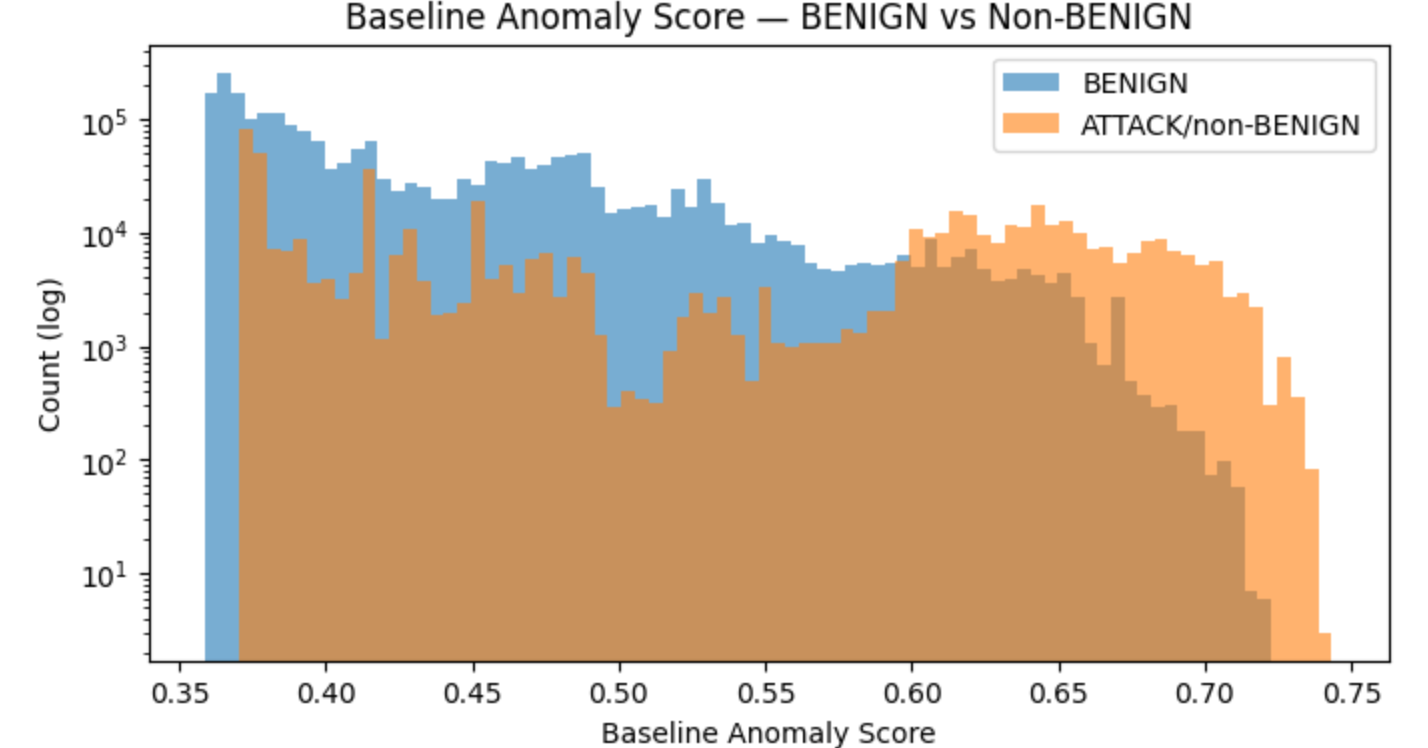
\includegraphics[width=0.5\linewidth]{imgs/base.png}
    \label{fig:placeholder}
\end{figure}
\noindent This graph shows that there are fewer BENIGN samples greater than around 0.6 score and the attack scores are shifted right with most scores between 0.55-0.72. This means that using the baseline anomaly model, it was able to assign lower scores to BENIGN traffic and higher scores to attacker traffic although there are some false positives and false negatives due to some overlap.
I then conducted analysis on the Zenodo CyberLab Honeynet Dataset. I conducted similar processing of data, feature extraction, and distribution plotting. Since this dataset has different data and features compared to the Network Intrusion Dataset, I used KMeans unsupervised learning to optimize clustering for a new attacker behavior model.
\begin{figure}[H]
    \centering
    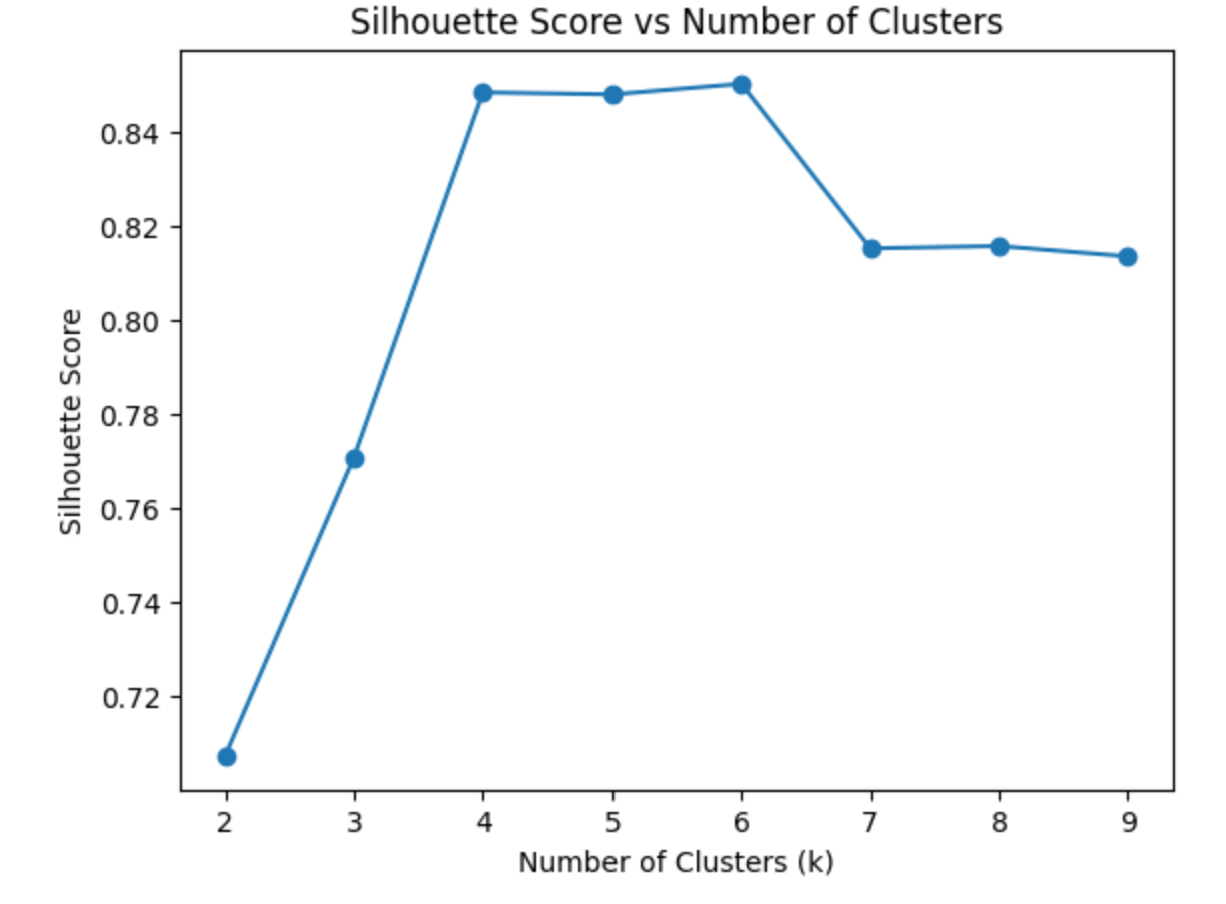
\includegraphics[width=0.5\linewidth]{imgs/sil.png}
    \label{fig:placeholder}
\end{figure}\begin{figure}[H]
    \centering
    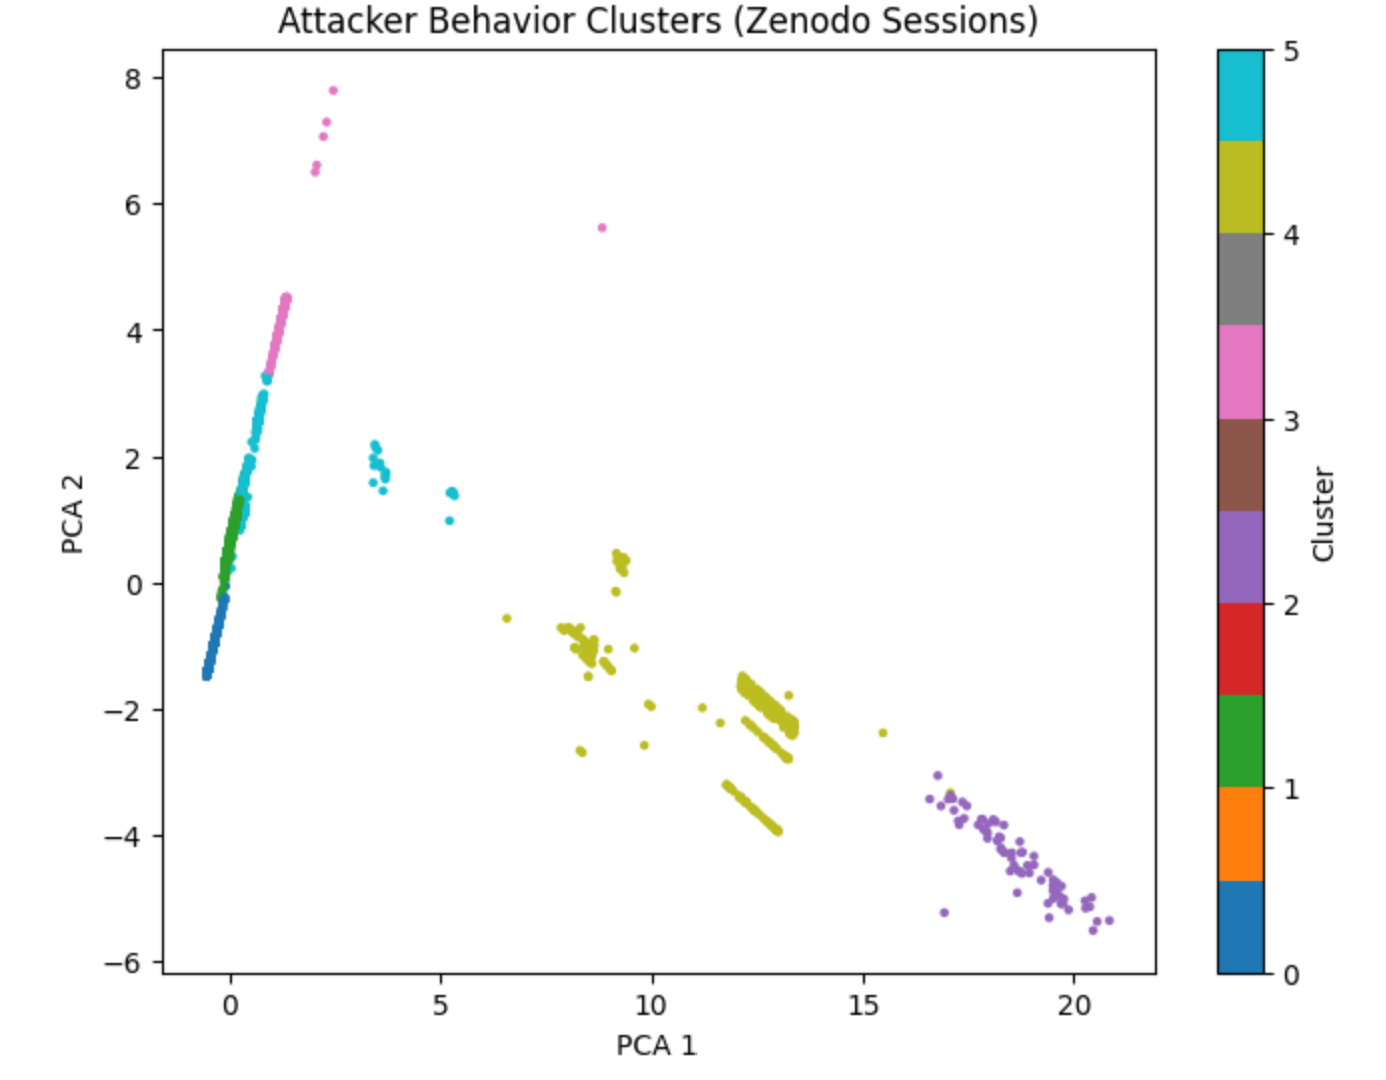
\includegraphics[width=0.5\linewidth]{imgs/cluster.png}
    \label{fig:placeholder}
\end{figure}
\noindent These graphs show that this dataset separates into well defined behavior groups. I then started a new Jupyter Notebook to write a skeleton pipeline for our project that we can adjust later on once we get our data from the honeypots where it expects Cowrie logs and converts them in session level feature tables that will be used for anomaly detection, attacker clustering, behavioral profiling, and supervised classification.
\subsection{Week of 3/2/2026}
This week I explored supervised learning for classification on the CIC-IDS dataset. I load in the data and clean the columns then plot the distributions of different attack types. We build two matrices with the target variable (y) and the feature matrix (X). I split the data into train/val/test using random stratified split. I used logistic regression and random forest to test which had the best results and settled on random forest which reached a validation and test accuracy of 99\%. 
\begin{figure}[H]
    \centering
    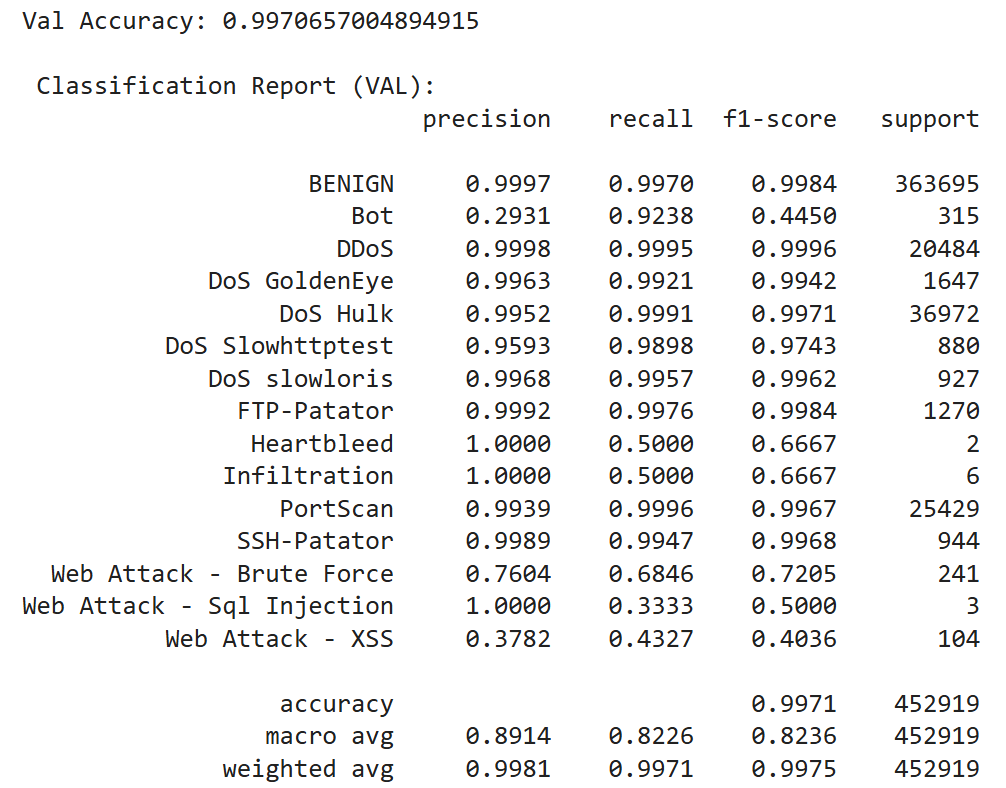
\includegraphics[width=0.7\linewidth]{imgs/val.png}
    \label{fig:placeholder}
\end{figure}
\begin{figure}[H]
    \centering
    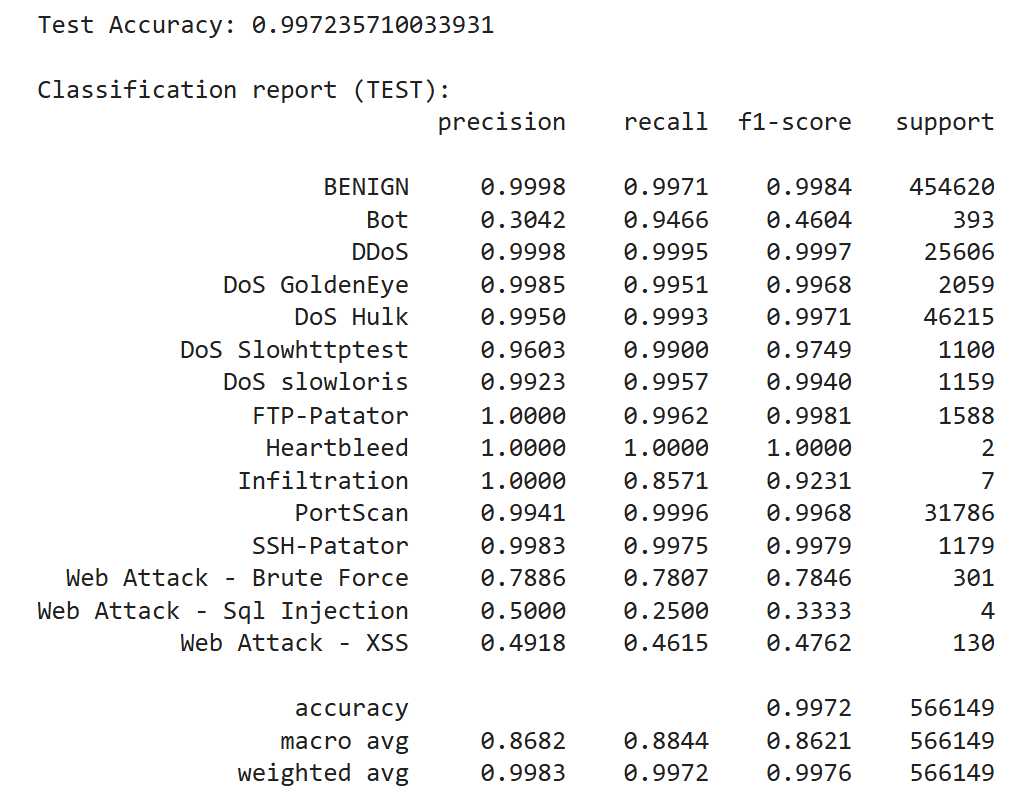
\includegraphics[width=0.7\linewidth]{imgs/test.png}
    \label{fig:placeholder}
\end{figure}
As the scrum master, I also worked on the early status report by planning out all of our expected sprints for Senior Design 1 and Senior Design 2. I added in all of our Jira and Agile Event information including the scrum reviews and plannings. 
\section{Journals}
\subsection{Journal 1}
\indent\indent This week, I organized our team's workflow in Jira by researching purpose and use of epics, stories, tasks, and subtasks by using online documentation and the PowerPoints in canvas. After this weeks meeting, I added new sprint tasks and assigned them on Jira based on each role's responsibilities. I set up our group's Design Proposal \& Team Contract and the Early Status Report documentation by creating a template with the table of contents based on the assignment requirements on canvas so everyone can start working on it. I added a READ.me and a scrum/meeting documentation on our GitHub so the team has access to view our minutes at anytime.
\\\indent For my machine learning and threat analysis role, I researched how they are applied in cybersecurity in clustering and anomaly detection. I concluded that building an effective pipeline requires things like session duration, command and prompt counts, and behavioral patterns. These features will be important in our project to help identify attack patterns, detect abnormal sessions, and possibly predict attacks down the line after our model is trained. I used various resources like academic papers, online documentation, and videos from IBM Technology to better my understanding during my research process.  I have no current blockers and next week I plan to work on protyping by writing up a structured framework for the pipeline including preprocessing steps in taking in the data, computing features, and plotting the distributions. I will use synthetic or test inputs to ensure everything works properly so we can integrate the real data later on.
\subsection{Journal 2}
\indent\indent This week, I worked on Jupyter Notebook to develop infrastructure for loading, processing, and analyzing two datasets that is related to our project. I analyzed the Network Intrusion dataset by merging all the data into one dataframe, extracted session level features, and trained it using the Isolation Forest model to establish baseline behavior. The model then assigned anomaly scores to normal and attack traffic where the attack traffic received higher scores meaning they far differentiate from the normal traffic baseline. For behavior modeling, I processed the Zenodo CyberLab Honeynet and performed similar feature extraction and distribution analysis process. I applied KMeans clustering to identify distinct behavioral groupings in the data. Afterwards, I began building a skeleton base pipeline to process Cowrie logs to convert them into session feature tables which is what we will be using for our project. I will be able to adjust the inputs and formatting once we began to collect our own honeypot data.
\\\indent My current blocker is that there is a lack of high-quality dataset for everything that our team wants to test. I wanted this dataset to build a baseline and for testing, but not all datasets have features such as password and commands due to security reasons. We may need to just wait till we collect enough data or use synthetic ones. Next week, I will work on building building a base training/testing structure of behavior modeling for after the data preprocessing of our honeypot data. I will also experiment with supervised learning approaches to classify attack types and research labeling strategies besides manual labeling to try and reduce time.
\subsection{Journal 3}
\indent \indent This week, I worked on the machine learning portion of the project by exploring and experimenting with supervised classification on the CIC-IDS dataset which is a similar dataset that we will produce, but it contains attack type labels. I'm able to use the labels to train the model then classify new data. I loaded the data and analyzed the columns of different features and attack types and plotted the distributions. We are able to visualize how many of each type of data occurred. I then created a feature matrix (X) and target variable (y) matrix and split the data into train/val/test using random stratified split. I trained and compare the logistic regression and random forest classifiers to get the best result. I selected random forest since it reached a validation and test accuracy of 99\%. This contributes to our project because it tells us that if we figure out the labeling information on our dataset, we can add classification analysis and detection to our project. 

\indent I also contributed to the early status report. As the scrum master, I planned our expected sprints for both Senior Design 1 and senior Design 2 by creating a table overview then a further in depth description of tasks and role specific objectives. I organized our Jira and Agile event information and added scrum planning and review minutes to the document as well. We have concluded that the supervised classification will become a stretch goal and instead, I will focus on behavioral analysis and clustering. I currently have no blockers and next week I plan to work on feature extraction, behavior analysis, and the pipeline for our cowrie logs that our honeypot has collected. 
\end{document}
